\documentclass[tikz,border=4pt]{standalone}
\usepackage{fontspec}
\setmainfont{Times New Roman}
\usetikzlibrary{arrows.meta,positioning,calc,fit,backgrounds}
\definecolor{ink}{HTML}{263747}
\definecolor{blue}{HTML}{27658E}
\definecolor{orange}{HTML}{B26724}
\definecolor{gray}{HTML}{65717C}
\DeclareMathSizes{8}{8}{6}{5.2}
\DeclareMathSizes{8.5}{8.5}{6}{5.2}
\DeclareMathSizes{9}{9}{6}{5.2}
\DeclareMathSizes{10}{10}{7}{5.2}
\begin{document}
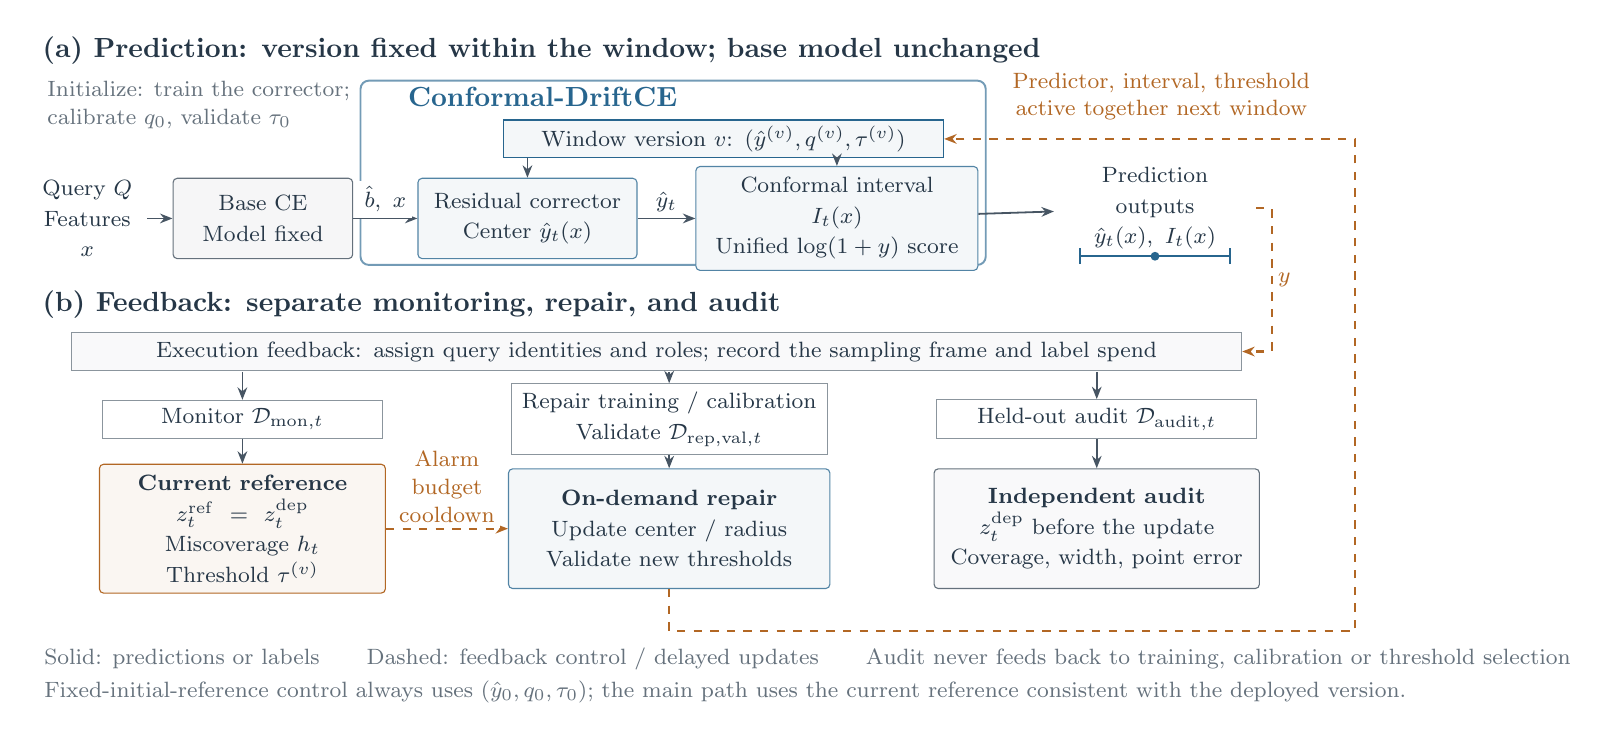
\begin{tikzpicture}[
 font=\fontsize{8.5}{11}\selectfont,text=ink,
 box/.style={draw=blue!80,fill=blue!5,rounded corners=1.5pt,minimum height=1.02cm,align=center,inner sep=4pt},
 data/.style={draw=gray!75,fill=white,align=center,inner sep=3pt,minimum height=.48cm},
 arr/.style={-{Stealth[length=4.5pt,width=3.5pt]},draw=ink!85,line width=.65pt},
 fb/.style={-{Stealth[length=4.5pt,width=3.5pt]},draw=orange,line width=.75pt,dashed},
 lab/.style={font=\fontsize{8}{10}\selectfont,fill=white,inner sep=2pt,align=center}
]
\node[anchor=west,font=\bfseries] at (.1,4.52) {(a) Prediction: version fixed within the window; base model unchanged};
\draw[draw=blue!65,rounded corners=3pt,line width=.7pt] (4.26,1.80) rectangle (12.20,4.14);
\node[anchor=west,text=blue,font=\bfseries] at (4.74,3.94) {Conformal-DriftCE};
\node[align=left,anchor=west,text=gray,font=\fontsize{8}{10}\selectfont] at (.16,3.83)
 {Initialize: train the corrector;\\calibrate $q_0$, validate $\tau_0$};
\node[data,draw=blue,fill=blue!5,text width=5.45cm,inner sep=2pt] (dep) at (8.87,3.40)
 {Window version $v$: $(\hat y^{(v)},q^{(v)},\tau^{(v)})$};
\node[align=center,text width=1.28cm] (query) at (.79,2.39) {Query $Q$\\Features $x$};
\node[box,draw=gray,fill=gray!6,text width=2.0cm] (base) at (3.02,2.39) {Base CE\\Model fixed};
\node[box,text width=2.5cm] (center) at (6.38,2.39) {Residual corrector\\Center $\hat y_t(x)$};
\node[box,text width=3.3cm] (interval) at (10.31,2.39) {Conformal interval\\$I_t(x)$\\Unified $\log(1+y)$ score};
\node[align=center,text width=2.32cm] (output) at (14.35,2.52) {Prediction outputs\\$\hat y_t(x),\ I_t(x)$};
\draw[blue,line width=.7pt] (13.40,1.91)--(15.30,1.91);
\draw[blue,line width=.7pt] (13.40,1.81)--(13.40,2.01);
\draw[blue,line width=.7pt] (15.30,1.81)--(15.30,2.01);
\fill[blue] (14.35,1.91) circle (1.6pt);
\draw[arr] (query)--(base);
\draw[arr] (base)--node[lab,above] {$\hat b,\ x$}(center);
\draw[arr] (center)--node[lab,above] {$\hat y_t$}(interval);
\draw[arr] (interval)--(output);
\draw[arr] (center.north |- dep.south)--(center.north);
\draw[arr] (interval.north |- dep.south)--(interval.north);
\node[anchor=west,font=\bfseries] at (.10,1.30) {(b) Feedback: separate monitoring, repair, and audit};
\node[data,fill=gray!4,text width=14.65cm] (feedback) at (8.02,.70)
 {Execution feedback: assign query identities and roles; record the sampling frame and label spend};
\draw[fb] (output.east)--(15.83,2.52)--node[lab,right,text=orange] {$y$}(15.83,.70)--(feedback.east);
\node[data,text width=3.35cm] (mondata) at (2.76,-.16) {Monitor $\mathcal D_{{\rm mon},t}$};
\node[data,text width=3.80cm] (repdata) at (8.18,-.16) {Repair training / calibration\\Validate $\mathcal D_{{\rm rep,val},t}$};
\node[data,text width=3.85cm] (auditdata) at (13.61,-.16) {Held-out audit $\mathcal D_{{\rm audit},t}$};
\draw[arr] (2.76,.44)--(mondata.north);
\draw[arr] (8.18,.44)--(repdata.north);
\draw[arr] (13.61,.44)--(auditdata.north);
\node[box,draw=orange,fill=orange!6,text width=3.35cm,minimum height=1.52cm] (monitor) at (2.76,-1.55)
 {\textbf{Current reference}\\$z_t^{\rm ref}=z_t^{\rm dep}$\\Miscoverage $h_t$\\Threshold $\tau^{(v)}$};
\node[box,text width=3.80cm,minimum height=1.52cm] (repair) at (8.18,-1.55)
 {\textbf{On-demand repair}\\Update center / radius\\Validate new thresholds};
\node[box,draw=gray,fill=gray!4,text width=3.85cm,minimum height=1.52cm] (audit) at (13.61,-1.55)
 {\textbf{Independent audit}\\$z_t^{\rm dep}$ before the update\\Coverage, width, point error};
\draw[arr] (mondata)--(monitor);
\draw[arr] (repdata)--(repair);
\draw[arr] (auditdata)--(audit);
\draw[fb] (monitor.east)--node[lab,above,text=orange] {Alarm\\budget\\cooldown}(repair.west);
\draw[fb] (repair.south)--(8.18,-2.85)--(16.89,-2.85)--(16.89,3.40)--(dep.east);
\node[lab,text=orange] at (14.43,3.94) {Predictor, interval, threshold\\active together next window};
\node[anchor=west,text=gray,font=\fontsize{8}{10}\selectfont] at (.12,-3.20)
 {Solid: predictions or labels\qquad Dashed: feedback control / delayed updates\qquad Audit never feeds back to training, calibration or threshold selection};
\node[anchor=west,text=gray,font=\fontsize{8}{10}\selectfont] at (.12,-3.62)
 {Fixed-initial-reference control always uses $(\hat y_0,q_0,\tau_0)$; the main path uses the current reference consistent with the deployed version.};
\end{tikzpicture}
\end{document}
